\begin{frame}{What is News recommendation?}
\framesubtitle{Why do we need to care about News recommendation?}
\begin{itemize}
    \item  A News recommendation system helps users to find the articles that are most interesting to them.
    \item News recommendation systems must be able to handle the challenge of fresh content, i.e., breaking news that hasn’t yet been viewed by many readers.
    \item Online services, news aggregation services, such as Google News can provide overwhelming volume of content than the amount that users can digest.
\end{itemize}
\end{frame}



\begin{frame}{RELATED WORK}
  \framesubtitle{News recommendation algorithms}
  Conventional news recommendation methods can be divided into three categories:
  \begin{itemize}
      \item Content-based methods will maintain news term frequency features (e.g., TF-IDF) and user profiles (based on historical news). Then, recommender will select news that is more similar to user profile.
      \item Collaborative filtering methods usually make rating prediction utilizing the past ratings of current user or similar users, or the combination of these two.
      \item To combine the advantages of the former two groups of methods, hybrid methods are further proposed to improve the user profile modeling.
  \end{itemize}
 
\end{frame}


\begin{frame}{Major drawbacks of the previous work}
   \begin{itemize}
       \item They only try to model current reward (e.g., Click Through Rate).
       \item Very few studies consider to use user feedback other than click / no click labels (e.g., how frequent user returns) to help improve recommendation.
       \item These methods tend to keep recommending similar news to users, which may cause users to get bored.
       \item They use discrete user log to represent state and hence can not be scaled to large systems.
\end{itemize}
\end{frame}

\begin{frame}{State-of-art reinforcement learning methods}
   \begin{itemize}
       \item State-of-art reinforcement learning methods usually apply the simple $\epsilon$-greedy strategy or Upper Confidence Bound (UCB) (mainly for Multi-Armed Bandit methods). 
       \item However, both strategies could harm the recommendation performance to some extent in a short period. 
       \item $\epsilon$ -greedy strategy may recommend the customer with totally unrelated items
       \item UCB can not get a relatively accurate reward estimation for an item until this item has been tried several times.
\end{itemize}
\end{frame}


\begin{frame}{User Behaviour}
        \begin{figure}
            \centering
            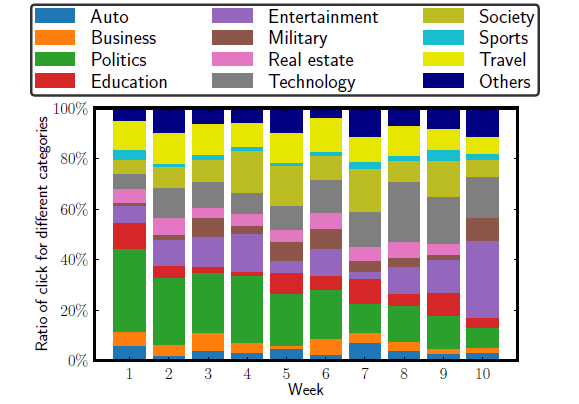
\includegraphics[scale = 0.6]{PPT/figure 1.png}
            \caption{Distribution of clicked categories of an active user
in ten weeks. User interest is evolving over time.}
        \end{figure}
\end{frame}


\begin{frame}{How is this method different?}
   \begin{itemize}
       \item In this paper, they propose a Deep Q-Learning based recommendation framework, which can model future reward explicitly.
       \item More information than click / no click label.
       \item In contrast to MAB-based methods, MDP-based methods can not only capture the reward of current iteration, but also the potential reward in the future iterations.
      \item Partial MDP can not scale to large dataset.
      \item They propose a MDP framework with continuous state and action representation.
\end{itemize}
\end{frame}






% \begin{frame}{Deep Reinforcement Recommendation System}
% 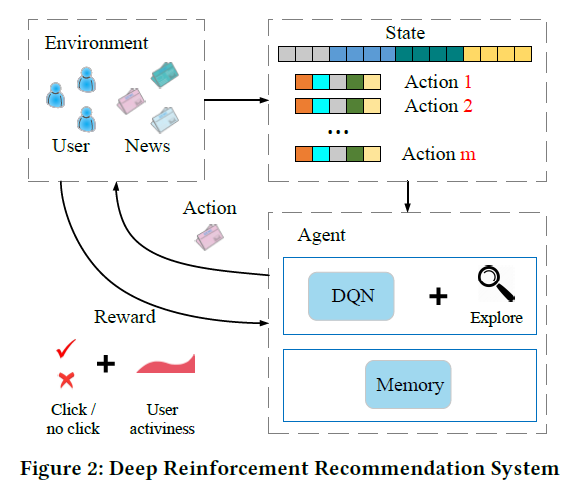
\includegraphics[height=6.8cm]{figure 2.png}
% \centering
% \end{frame}

% \begin{frame}{Deep Reinforcement Recommendation System}
% \begin{itemize}

%  \item In order to better model the dynamic nature of news characteristics and user preference, Deep Q-Learning (DQN) framework has been used.
%       \item This framework uses a DQN structure and can easily scale up.
%       \item The framework consider user return as another form of user feedback information, by maintaining an activeness score for each user.
%       \item The framework consider multiple historical return interval information to better measure the user feedback.
%       \item The model can estimate user activeness at any time (not just when user returns). This property enables the experience replay update used in DQN.
%       \item By applying a Dueling Bandit Gradient Descent (DBGD) method for exploration, by choosing random item candidates in the neighborhood of the current recommender, the strategy avoid recommending totally unrelated items and hence maintain better recommendation accuracy.
%       \end{itemize}
% \end{frame}

%merge the next three and form two slides



 
%  \begin{frame}{Notations}
% 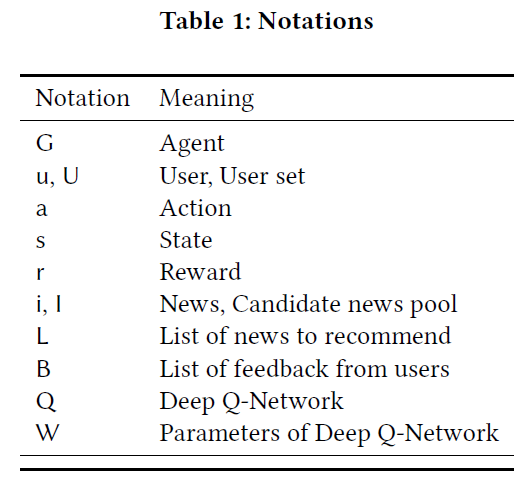
\includegraphics[height=6.8cm]{figure 3.png}
% \centering
% \end{frame}



